The aerodynamics of the rocket are essential to the behaviour of a launch vehicle, as they enact both forces and moments on the body. The chosen method is to use lift and drag coefficients, which vary with Mach number and angle of attack. As experiemtnal data on \textit{Space X}'s or \textit{Blue Origin}'s rockets is confidental, the legacy data of the Wernher von Braun's V2 rocket from WW2 is used to provide a benchmark for preliminary modelling. This can be improved in later studies, as the V2 (\autoref{fig:V2_rocket}) is obviously a lot different to modern launch vehicles. This section discusses the trends observed in the V2 aerodynamic coefficient curves, shown in \autoref{fig:V2_curves} (\cite{sutton_rocket_2016}), and relates them to the governing flow physics across subsonic, transonic, and supersonic conditions.


\begin{figure}[H]
    \centering
    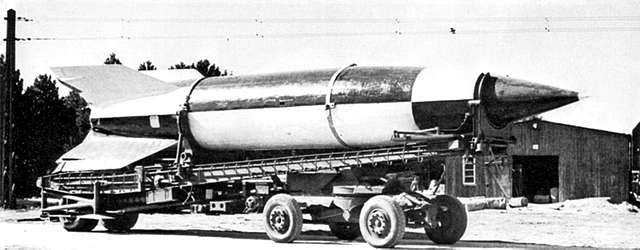
\includegraphics[width=0.75\linewidth]{figures/LiteratureStudy/V2_image.jpg}
    \caption{V2 rocket on Meillerwagen.\footnote{\url{https://timelessmoon.getarchive.net/media/v-2-rocket-on-meillerwagen-9effc8} (Accessed: 22 May 2025)}}
    \label{fig:V2_rocket}
\end{figure}

During the subsonic regime, under Mach 0.8, the drag is independent of the Mach number as compressibility effects are minimal. The lift coefficient has an initial increase with Mach number before a decrease, with the magnitude of the change observed being greater at higher angles of attack as the circulation around the rocket increases.

For the transonic regime, between Mach 0.8 and 1.2, shock waves begin to form and propagate over the rocket's surface, causing \textit{drag divergence}. Resulting in a rapid rise in drag approaching maximum drag and lift at 1.2. Strong shock and boundary layer interactions cause unsteady flow inducing the coefficient's rise.

\begin{figure}[H]
    \centering
    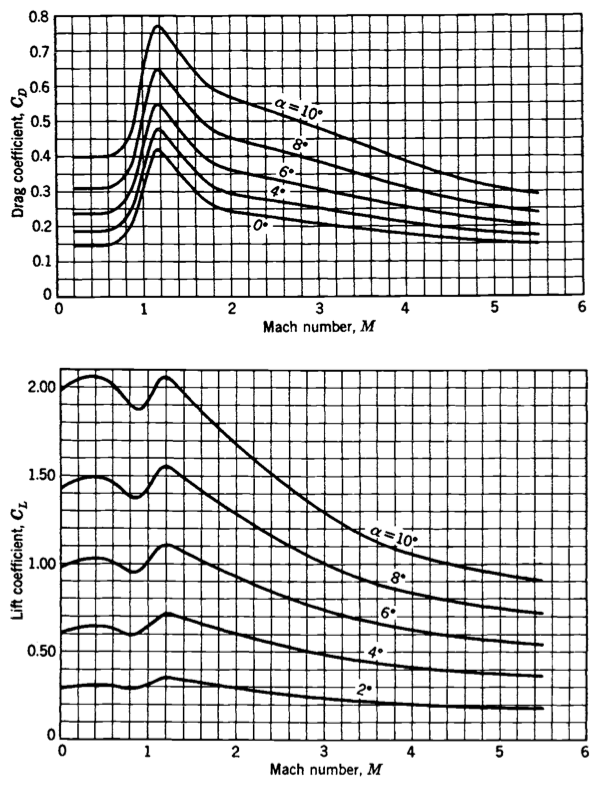
\includegraphics[width=0.75\linewidth]{figures/LiteratureStudy/V2-lift-drag-coefficient (1) (2).png}
    \caption{V2 rocket lift and drag coefficient curves (\cite{sutton_rocket_2016}).}
    \label{fig:V2_curves}
\end{figure}

The center of pressure (CoP) is the point on the rocket's body where the resultant aerodynamic force acts, in our case the lift and drag forces. \cite{TIR-33} states that a rocket during has aerodynamic stability if its center of pressure (CoP) is behind its center of gravity (CoG). A rocket may deviate for instance due to wind gusts, causing an increased angle of attack, a stable rocket will correct for this by forcing it back to zero over time. As a result, the center of pressure of the rocket is placed such that the rocket is aerodynamically stable during ascent and descent. A higher fidelity model for the center of pressure is not considered, as data on the V2 missile's center of pressure change with angle of attack and Mach number was not found. So the chosen CoP model cannot be validated, a constant center of pressure is taken.

The lift and drag coefficients of \autoref{fig:V2_curves} are converted to forces, lift and drag, through \autoref{eq:lift_drag}. Where the area $S$ is the cross-sectional area of the rocket, so $S = \pi \cdot r_r^2$, and the dynamic pressure is $q = \frac{1}{2} \cdot \rho \cdot V^2$.

\begin{equation}
\begin{aligned}
    L =& \frac{1}{2} \cdot \rho \cdot V^2 \cdot C_L \cdot S \\
    D =& \frac{1}{2} \cdot \rho \cdot V^2 \cdot C_D \cdot S
\end{aligned}
\label{eq:lift_drag}
\end{equation}

For the ascent phase, the center of pressure is behind the center of gravity, this gives the freebody diagram \autoref{fig:aero_reference_frames}, with angle of attack $\alpha$ the difference between the pitch and the flight path angle. Here two frames are present $(x',y')$ which is the initial reference frame, which is launchpad reference frame; x horizontal and right upward, translated to act at the rocket's center of gravity.$(x'',y'')$ is the body frame. From this freebody diagram the equations of motion can be derived, \autoref{eq:aero_forces_ascent}.

\begin{equation}
\begin{aligned}
    F_{x''} =& -L \cdot \cos(\alpha) -D\cdot\sin(\alpha) \\
    F_{y''} =& L \cdot \sin(\alpha) - D \cdot \cos(\alpha) \\
    M_z =& (d_{cg} - d_{cp}) \cdot ( -L \cdot \cos(\alpha) -D\cdot\sin(\alpha))
\end{aligned}
\label{eq:aero_forces_ascent}
\end{equation}

The center of pressure location is checked to find it's stable position with respect to the center of gravity. When an angle of attack is formed a negative aerodynamic moment is desired to correct the angle of attack. \autoref{eq:stability_ascent} derives the moments derivative with respect to angle of attack, before applying the small angle approximation. With a small $\alpha$ then $L\cdot \alpha << D$, and with the rest of the factors positive, the moment is restored.

\begin{equation}
\begin{aligned}
    \frac{dM_z}{d\alpha} =& (d_{cp} - d_{cg}) \cdot (L \cdot \sin(\alpha) -D \cdot \cos(\alpha) - C_{L_\alpha} q \cdot S\cdot \cos(\alpha) - C_{D_\alpha} \cdot q \cdot S \sin(\alpha)) \\
    =& (d_{cp} - d_{cg}) \cdot (L \cdot \alpha - D - C_{L_\alpha}\cdot q \cdot S - C_{D_\alpha} \cdot q \cdot S \cdot \alpha)
\end{aligned}
\label{eq:stability_ascent}
\end{equation}

The descent reference from of \autoref{fig:aero_reference_frames} is used to derive the body frame forces from the aerodynamics in \autoref{eq:descent_aero}. The effective angle of attack denotes the descent angle of attack which is found using \autoref{eq:eff_alpha}.

\begin{equation}
    \alpha_{eff} = \gamma - (\theta + \pi)
\label{eq:eff_alpha}
\end{equation}
        
\begin{equation}
\begin{aligned}
    F_{x''} =& -D \cdot \sin(\alpha_{eff}) - L \cdot \cos(\alpha_{eff}) \\
    F_{y''} =& D \cdot \cos(\alpha_{eff}) - L \cdot \sin(\alpha_{eff}) \\
     M_z =& (d_{cg} - d_{cp}) \cdot( -D \cdot \sin(\alpha_{eff}) - L \cdot \cos(\alpha_{eff}))
\end{aligned}
\label{eq:descent_aero}
\end{equation}

With the center of pressure now moved to the top of the rocket, the aerodynamic stability is checked in \autoref{eq:stability_descent}. For aerodynamic stability a positive restoring moment is required to minimise the angle of a. \autoref{eq:stability_descent} derives the moment derivative with respect to effective angle of attack before the small angle approximation is applied. A small angle of will make $L \cdot \alpha_{eff} << D$ so the applied moment is positive, as the rest of the terms are positive.

\begin{equation}
\begin{aligned}
    \frac{dM_z}{d\alpha_{eff}} =& (d_{cp} - d_{cg}) \cdot (C_{D_{\alpha_{eff}}} \cdot q \cdot S \cdot \sin(\alpha_{eff}) + C_{L_{\alpha_{eff}}} \cdot q \cdot S \cdot \cos(\alpha_{eff}) + D \cdot \cos(\alpha_{eff}) - L \cdot \sin(\alpha_{eff})) \\
    =& (d_{cp} - d_{cp}) \cdot (C_{D_{\alpha_{eff}}} \cdot q \cdot S \cdot \alpha_{eff} + C_{L_{\alpha_{eff}}} \cdot q \cdot S + D - L \cdot \alpha_{eff})
\end{aligned}
\label{eq:stability_descent}
\end{equation}

The translate into the inertia frame the transformations of \autoref{eq:inertial_aero} are performed, for descent and ascent.

\begin{equation}
\begin{aligned}
    F_{x'} =& F_{y''} \cdot \cos(\theta) + F_{x''} \cdot \sin(\theta) \\
    F_{y'} =& F_{y''} \cdot \sin(\theta) - F_{x''} \cdot \cos(\theta)
\end{aligned}
\label{eq:inertial_aero}
\end{equation}    

\begin{figure}[H]
    \centering
    \begin{subcaptionbox}{Ascent.}[0.45\linewidth]
        {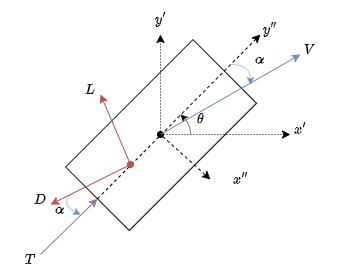
\includegraphics[width=\linewidth]{figures/LiteratureStudy/AerodynamicReference_ascent.png}}
        \label{fig:ascent_aero}
    \end{subcaptionbox}
    \hfill
    \begin{subcaptionbox}{Descent.}[0.45\linewidth]
        {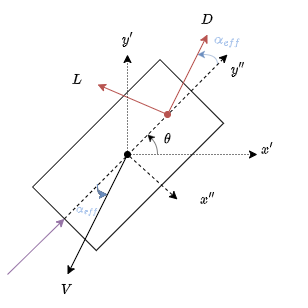
\includegraphics[width=\linewidth]{figures/LiteratureStudy/AerodynamicReference_descent (1).png} (1).png}
        \label{fig:descent_aero}
    \end{subcaptionbox}
    \caption{Aerodynamic Reference frames}
    \label{fig:aero_reference_frames}
\end{figure}